\chapter{Modelling, Data, and Simulation}
\label{cha:model}

\minitoc

\section{Introduction}

After describing the state-of-the-art, this chapter presents the models, data, and simulation tools used in this thesis. First, we focus on the model describing the offline and online scheduling problem. We explain what kind of information is exchanged between offline and online. After the model, we introduce the traces used in the experiments. These traces emulate a real environment regarding workload, weather, and platform. Finally, we detail the simulation tools, explaining the modifications needed to create the experimental environment.

\section{Model}

As presented in Chapter \ref{cha:related_work}, a gap in the state-of-the-art is the mix of offline and online. Figure \ref{fig:model} illustrates the architecture proposed by the Datazero2 project, mixing both decision levels \cite{Datazero}. Since this work is part of this project, we use the same architecture. There are four main modules: IT Decision Module (ITDM), Power Decision Module (PDM), Negotiation Module (NM), and Online Decision Module (ODM). ITDM, PDM, and NM are responsible for the offline decisions, and ODM manages the online actions. This thesis focuses on the Online Decision Module. However, we present in the following sections the optimizations made in offline modules to provide the data needed by ODM since we propose a mix between offline and online decisions.

Besides these four modules, Datazero2 also includes an event generator and a metronome. Both components are essential for the simulations. Event generator simulates the real events of a data center, such as job submissions, weather conditions, etc. It simply reads a file and sends the data to the bus. The metronome synchronizes the simulation messages. So, every component waits for the time evolution from the metronome. This thesis does not detail these components, concentrating on the decision modules and their interactions.

\begin{table*}[!htb]
\centering
% \scriptsize
\caption{General notations.}
\label{tab:notation_system}
\begin{tabular}{l|l}
    \hline
    Notation & Description \\\hline\hline
    % System
    $t$ & Time step (int)\\
    $T$ & Last time step (int)\\
    $\Delta t$ & Time step length (s)\\
    $T_{w}$ & Time window length (s)\\
    $P_{load}$ & Estimated power demand (kW)\\
    $u_{load}$ & Uncertainty of $P_{load}$\\
    $P_{prod}$ & Power production by all sources (kW)\\
    $P_{renew}$ & Power delivered by renewable sources (kW)\\
    $u_{renew}$ & Uncertainty of $P_{renew}$\\
    \hline
\end{tabular}
\end{table*}

Table \ref{tab:notation_system} presents the general notations and each following section introduces its own notations. Both offline and online use the time division from Figure \ref{fig:time_window}. The time window is the horizon of the offline plan. Offline considers the time window to define how far to predict weather and workload. In addition, it uses the time window to determine the planned actions. Our model divides the time window into several time steps, as represented in Figure \ref{fig:time_window} by the different $t$. The actions for power and server are constant inside the time step. For example, if a server is at some state in step $t=0$, it will remain at this state during the step duration.

\begin{figure}[!htb]
    \centering
    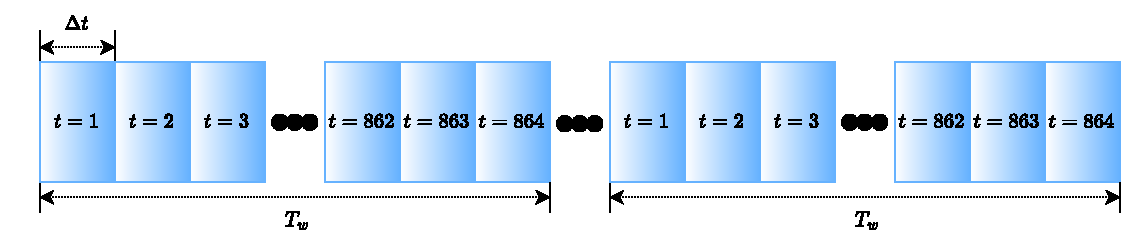
\includegraphics[scale=0.75]{Images/Model/Time window.pdf}
    \caption[Time window definition]{Time window definition. It gives an example of a time window of 3 days and a time step of 5 minutes. Each hour has 12 steps of 5 minutes (60 minutes / 5 minutes = 12 steps). So, three days have 864 steps (12 steps $\times$ 24 hours $\times$ 3 days = 864 steps).}
    \label{fig:time_window}
\end{figure}

\subsection{Offline Decision Modules}
\label{sec:offline_modules}

This section starts presenting the offline decision modules. First, we demonstrate how PDM and ITDM agree on a power envelope through NM. Then, we explain the power decisions from PDM, resulting in a power plan. Finally, we detail the ITDM, which defines the IT plan.

\subsubsection{Negotiation (NM)}
% Negotiation is a crucial step in Datazero2 architecture. A renewable-only data center introduces several constraints and decision variables. On the PDM side, it must approximate demand and production while considering long-term storage elements. For example, PDM can provide more power from hydrogen in a case with low renewable generation. However, PDM must evaluate the impact of its actions since the energy of the storage is finite. On the other hand, ITDM maximizes the Quality of Service. Thus, it demands more energy to run more servers at faster speeds. NM is between PDM and ITDM, trying to find an agreement. NM works iteratively. On each iteration, both PDM and ITDM propose a power envelope to NM, considering the objective of each module. A power envelope is a time series of the power production from the sources in a time window. While PDM tries to reduce the power envelope to control the storage, ITDM increases it to run more jobs faster. NM compares both envelope propositions and returns a new one. Then, each module verifies if they can use the proposed power envelope. They run several iterations until both agree or reach a timeout.

The negotiation Module is between PDM and ITDM, trying to find an agreement about the power profile. Since this thesis focuses on the online part, we simplify this process. We implemented the negotiation in three steps. First, ITDM proposes a power envelope $P_{load}$ based on the energy demanded to run a predicted workload. $P_{load}$ is a prediction from ITDM. We do not include it in this model, but we present in the following chapters how we generated it. Then, PDM takes this envelope and runs its optimization. It can degrade the power envelope to meet its objectives, resulting in a new power envelope $P_{prod}$. Finally, ITDM takes the PDM power production and finds the best server configuration that meets it. The following sections present the PDM and ITDM optimizations.

\subsubsection{Power Decision Module (PDM)}
Table \ref{tab:notation_power} gives the notations for PDM. PDM plans the renewable source engagement to provide the energy needed to maintain the IT elements running. A renewable-only data center introduces several constraints in power generation. Therefore, PDM must approximate the demanded power while considering long-term storage elements. For example, it can use more energy coming from hydrogen during the winter, which has lower power production, compensating for this usage in the summer, which has higher power generation. On the other hand, PDM can degrade the provided energy due to a lack of energy from storage and estimated renewable. Previously, \citeauthor{haddad2019mixed} created the first model to solve this problem \cite{haddad2019mixed}. This thesis uses a similar model to PDM. Equation \ref{equ:model_energy} gives the power production from all renewable sources. Equation \ref{equ:renewable_power} indicates that $P_{renew}$ comes from wind and solar production. $P_{wt}(t)$, $P_{pv}(t)$, $P_{fc}(t)$, $P_{ez}(t)$, $P_{dch}(t)$, and $P_{ch}(t)$ are calculated using Equations \ref{equ:wind_turbines}, \ref{equ:panel_solar_with_temperature}, \ref{equ:hydrogen_fuel_cell}, \ref{equ:hydrogen_electrolyzer} and \ref{equ:battery_energy} from Section \ref{sec:related_work_electrical_elements}. Batteries are reversible, which means that they can charge ($P_{ch}(t)$) and discharge ($P_{dch}(t)$) energy. Similarly, hydrogen can be considered reversible using an electrolyzer to charge ($P_{ez}(t)$) and a fuel cell to discharge ($P_{fc}(t)$). 

\begin{table*}[!htb]
\centering
% \scriptsize
\caption{Notations for PDM.}
\label{tab:notation_power}
\begin{tabular}{l|l}
    \hline
    Notation & Description \\\hline\hline
    % Power
    $P_{wt}$ & Power delivered by wind turbines (kW)\\
    $P_{pv}$ & Power delivered by solar panels (kW)\\
    $P_{fc}$ & Power delivered by fuel cell (kW)\\
    $P_{ez}$ & Power put into electrolyzer to generate hydrogen (kW)\\
    $P_{dch}$ & Battery discharging power (kW)\\
    $P_{ch}$ & Battery charging power (kW)\\
    $\eta_{ch}$ & Battery charge efficiency (\%)\\
    $\eta_{dch}$ & Battery discharge efficiency (\%)\\
    $SoC$ & State of Charge (\%)\\
    $LoH$ & Level of Hydrogen (kg)\\
    $SoC_{max}$ & Maximal battery State of Charge (\%)\\
    $SoC_{min}$ & Minimal battery State of Charge (\%)\\
    $B_{size}$ & Size of the battery (kWh)\\
    $LoH_{max}$ & H2 tank limit (kg)\\
    $P_{dch_{max}}$ & Battery maximum discharging power (kW)\\
    $P_{ch_{max}}$ & Battery maximum charging power (kW)\\
    $P_{fc_{max}}$ & Fuel cell maximum charging power (kW)\\
    $P_{ez_{min}}$ & Electrolyzer minimum charging power (kW)\\
    $P_{ez_{max}}$ & Electrolyzer maximum charging power (kW)\\
    $SoC_{target}$ & Target State of Charge at the end of the time window (\%)\\
    $LoH_{target}$ & Target Level of Hydrogen at the end of the time window (kg)\\
    $rf$ & Relax factor (float) \\
    $P^{real}_{load}$ & Real power demand (kW)\\
    $P^{real}_{renew}$ & Estimated power demand (kW)\\
    \hline
\end{tabular}
\end{table*}

\begin{equation}
    \label{equ:model_energy}
    P_{prod}(t) = P_{renew}(t) + (P_{fc}(t) + P_{dch}(t) - P_{ez}(t) - P_{ch}(t)), \quad \forall 0 \le t \le T
\end{equation}

\begin{equation}
    \label{equ:renewable_power}
    P_{renew}(t) = P_{wt}(t) + P_{pv}(t), \quad \forall 0 \le t \le T
\end{equation}

$P_{ch}(t)$, $P_{dch}(t)$, $P_{ez}(t)$, and $P_{fc}(t)$ are the decision variables in Equation \ref{equ:model_energy}, since $P_{wt}(t)$ and $P_{pv}(t)$ come from wind speed and solar irradiance. As presented in Section \ref{sec:related_work_electrical_elements}, $SoC(t)$ depends on the charge $P_{ch}(t)$ and discharge $P_{dch}(t)$ (see Equation \ref{equ:battery_energy}), and $LoH(t)$ depends on the power of the electrolyzer $P_{ez}(t)$ and fuel cells $P_{fc}(t)$ (see Equation \ref{equ:hydrogen_level}). Regarding $SoC(t)$, the state of charge must be between the boundaries $SoC_{min}$ and $SoC_{max}$, as written in Equation \ref{equ:battery_boundaries}. These boundaries help to extend the battery lifespan \cite{xu2016modeling}.

\begin{equation}
    \label{equ:battery_boundaries}
    SoC_{min} \leq SoC(t) \leq SoC_{max}, \quad \forall 0 \le t \le T
\end{equation}

On the other hand, hydrogen only has the tank size as a boundary. So, Equation \ref{equ:hydrogen_boundaries} presents the level of hydrogen constraint.

\begin{equation}
    \label{equ:hydrogen_boundaries}
    0 \leq LoH(t) \leq LoH_{max}, \quad \forall 0 \le t \le T
\end{equation}

Considering the power to charge/discharge the batteries, both have upper limits. These boundaries avoid destroying the battery. So, we introduce constraints \ref{equ:discharge_boundary} and \ref{equ:charge_boundary}.

\begin{equation}
    \label{equ:discharge_boundary}
    0 \leq P_{dch}(t) \leq P_{dch_{max}}, \quad \forall 0 \le t \le T
\end{equation}

\begin{equation}
    \label{equ:charge_boundary}
    0 \leq P_{ch}(t) \leq P_{ch_{max}}, \quad \forall 0 \le t \le T
\end{equation}

Fuel cells and electrolyzers also have boundaries. While fuel cells have only a maximum limit, electrolyzers have an operating range. So, Equations \ref{equ:fuelcells_boundary} and \ref{equ:electrolyzer_boundary} present them.

\begin{equation}
    \label{equ:fuelcells_boundary}
    0 \leq P_{fc}(t) \leq P_{fc_{max}}, \quad \forall 0 \le t \le T
\end{equation}

\begin{equation}
    \label{equ:electrolyzer_boundary}
    P_{ez_{min}} \leq P_{ez}(t) \leq P_{ez_{max}}, \quad \forall 0 \le t \le T
\end{equation}

Another important constraint is the target hydrogen and battery level at the end of the time window ($SoC(T)$). Using only the previous constraints, the model can use all the power available in the energy storages, drying them but providing a high quality of service. However, Figure \ref{fig:time_window} shows that the time windows are chained. So, the next time window will not have energy in the storage. Therefore, we introduce these targets. So, the state of charge and level of hydrogen in the last step of the time window must respect Equations \ref{equ:soc_target} and \ref{equ:loh_target}. These targets can be the subject of another optimization or indicated by hand by the data center manager. Furthermore, the targets must consider the long-term perspective, such as seasons with lower/higher production, the peak of demand over an external event, etc. 

\begin{equation}
    \label{equ:soc_target}
    SoC(T) \ge SoC_{target}
\end{equation}

\begin{equation}
    \label{equ:loh_target}
    LoH(T) \ge LoH_{target}
\end{equation}

Finally, the objective is to approximate the power production to the power demand. So, Equation \ref{equ:load_production} shows the relation between demand ($P_{load}$) and generation ($P_{prod}$). The optimization finds a solution where the production is higher or equal to the demand. However, it can not match both in every case. Therefore, the model introduces a demand degradation using a relax factor ($rf$). With the relax factor equal to 0, it matches demand and production. Increasing the relax factor would reduce the power given to IT, impacting the QoS. Thus, the objective is reducing the relax factor, as presented in Equation \ref{equ:objective_function}.

\begin{equation}
    \label{equ:load_production}
    P_{prod}(t) \ge (1 - rf) \times P_{load}(t), \quad \forall 0 \le t \le T
\end{equation}

\begin{equation}
    \label{equ:objective_function}
    \mathbf{minimize}\ rf
\end{equation}

% \citeauthor{haddad2019mixed} presented a way to linearize this model, allowing it to be solved using MILP. This thesis used the \citeauthor{haddad2019mixed} proposition to solve it using MILP. 

% \begin{equation}
%     \label{equ:model_wind_turbines}
%     P_{WT}(t) = \begin{cases}
%         0 & v \leq v_{in} \text{ or } v(t) > v_{out} \\
%         P_{WT,rated} \times \frac{v^{3}(t) - v^{3}_{in}}{v^{3}_{rated} - v^{3}_{in}} & v_{in} < v(t) \leq v_{rated} \\
%         P_{WT,rated} & v_{rated} < v(t) \leq v_{out}
%     \end{cases}
% \end{equation}

% \begin{equation}
%     \label{equ:model_panel_solar_with_temperature}
%     P_{pv}(t) = P_{R,PV} \times (R / R_{ref}) \times \eta_{PV}
% \end{equation}

% \begin{equation}
%     \label{equ:model_battery_energy}
%     E_{bat}(t) = (E_{bat}(t-1) \times (1 - \sigma)) + (P_{ch}(t-1) \times \eta_{ch} \times \Delta t) - (P_{dch}(t-1) \times \eta_{dch} \times \Delta t)
% \end{equation}
% \begin{equation}
%     \label{equ:model_battery_state_of_charge}
%     SoC(t) = \frac{E_{bat}(t)}{C_{bat}} \times 100
% \end{equation}

% \begin{equation}
%     \label{equ:model_hydrogen_electrolyzer}
%     P_{ez}(t) \times \Delta t = \frac{HH_{h_{2}} \times Q_{ez}(t)}{\eta_{ez}}
% \end{equation}

% \begin{equation}
%     \label{equ:model_hydrogen_fuel_cell}
%     P_{fc}(t) \times \Delta t = LH_{h_{2}} \times Q_{fc}(t) \times \eta_{fc}
% \end{equation}

% \begin{equation}
%     \label{equ:model_hydrogen_level}
%     LoH(t) = LoH(t-1) + Q_{ez}(t-1) - Q_{fc}(t-1)
% \end{equation}

\subsubsection{IT Decision Module (ITDM)}

ITDM aims to maximize QoS, translating $P_{prod}(t)$ into server configuration. Table \ref{tab:notation_it} introduces the notations for ITDM. Server configuration means the CPU P-state of the servers. For each P-state, the server has a speed (in flops \cite{hunger2005floating}) and power consumption (in W). Table \ref{tab:servers} exemplifies this relation. The CPU frequency range is discrete, although some works define it to be continuous \cite{saha2012experimental}. ITDM must find the best combination of servers off and on at some speed that uses equal or less energy than the power envelope $P_{prod}(t)$. Thus, given a data center with $S$ servers, each server $s$ has a list of states $D_s$. Each state $d$ in $D_s$ has a speed $F_{s,d}$ and a power $P_{s,d}$. $D_{s,d}(t)$ is the boolean decision variable that indicates that the server $s$ is at state $d$ at step $t$. The sleep state has a different state $Dsl_{s}(t)$ which helps to identify the transition between sleeping and running. The transition between on$\rightarrow$off is called sedating and off$\rightarrow$on is waking.

\begin{table*}[!htb]
\centering
% \scriptsize
\caption{Notations for ITDM.}
\label{tab:notation_it}
\begin{tabular}{l|l}
    \hline
    Notation & Description \\\hline\hline
    $S$ & Servers (list) \\
    $N_{S}$ & Number of servers (int) \\
    $s$ & Server index (int) \\
    $D_s$ & States of server s (list) \\
    $N_{D_{s}}$ & Number of states of server s (int) \\
    $d$ & State index (int) \\
    $F_{s,d}$ & Speed of server $s$ at state $d$ (Flops)\\
    $P_{s,d}$ & Power of server $s$ at state $d$ (W)\\
    $D_{s,d}$ & Indicates that the server $s$ is at state $d$ (boolean)\\
    $Dsl_{s}$ & Indicates that the server $s$ is sleeping (boolean)\\
    $wa_s$ & Indicates if the server is waking, transiting from off$\rightarrow$on (boolean) \\
    $T_{wa_s}$ & Transition time from off$\rightarrow$on (s) \\
    $se_s$ & Indicates if the server is being sedate, transiting from on$\rightarrow$off (boolean) \\
    $T_{se_s}$ & Transition time from on$\rightarrow$off (s) \\    
    $E_{tot}$ & Energy total spent by the servers (J) \\
    $E_{run}$ & Energy spent by the running servers (J) \\
    $E_{wak}$ & Energy spent by waking the servers (J) \\
    $E_{sed}$ & Energy spent by sedating the servers (J) \\
    $E_{sle}$ & Energy spent by the sleeping servers (J) \\
    \hline
\end{tabular}
\end{table*}

\begin{table}[!htb]
\centering
\caption[Server definition example]{Server definition example. The power is for all server's processors busy. The values are from Grid5000's Parasilo server~\cite{dacosta:hal-03453537v1, dacostakeynote}.}
\label{tab:servers}
\begin{tabular}{c|c|c}
    \hline
    State        & Power (W) & Speed (Gflops) \\ \hline\hline
    0                       & 221.77                   & 38.4                          \\
    1                       & 216.77                   & 37.78                         \\
    2                       & 213.58                   & 36.93                         \\
    3                       & 208.90                   & 36.01                         \\
    4                       & 204.45                   & 34.72                         \\
    5                       & 200.62                   & 33.90                         \\
    6                       & 197.28                   & 32.84                         \\
    7                       & 192.49                   & 31.72                         \\
    8                       & 184.26                   & 30.63                         \\
    9                       & 182.04                   & 29.25                         \\
    10                      & 179.75                   & 27.93                         \\
    11                      & 176.70                   & 26.37                         \\
    12                      & 175.53                   & 25.01                         \\
    13 (sleep)              & 4.5                      & 0                             \\ \hline
\end{tabular}
\end{table}

First, Equation \ref{equ:one_state_only} ensures only one state per time $t$. The state can be anyone from $D_{s,d}$ to indicate a P-state, or $Dsl_{s}(t)$ to specify the sleep state. Since both variables are booleans (accepting only 0 or 1 values), summing them must be equal to 1 (at least one must be true). Both $D_{s,d}$ and $Dsl_{s}(t)$ are the only decision variables in the ITDM model.

\begin{equation}
    \label{equ:one_state_only}
    Dsl_{s}(t) + \sum_{d=0}^{N_{D_{s}}} D_{s,d}(t) = 1, \quad \forall 0 \le t \le T, \forall 0 \le s \le N_{S}
\end{equation}

Then, we must model the sedating and waking transitions. These transitions take time and spend energy. During these transitions, the servers are unavailable to run jobs. So, Equations \ref{equ:transition_wake} and \ref{equ:transition_sedating} model the waking transition (off$\rightarrow$on) and the sedating transition (on$\rightarrow$off), respectively. For example, Equation \ref{equ:transition_wake} verifies if the previous state is sleeping ($Dsl_{s}(t-1) = 1$) and now is not sleeping ($Dsl_{s}(t) = 0$). So the result of $Dsl_{s}(t-1) - Dsl_{s}(t)$ will be $1$, which indicates that the server $s$ is waking. If both are $0$ or $1$, the result is $0$, implying that the server is not transiting. If the previous state is not sleeping ($Dsl_{s}(t-1) = 0$) and now is sleeping ($Dsl_{s}(t) = 1$), the result will be $-1$. However, the $\max (0)$ function will put 0 as $wa_s(t)$. Equation \ref{equ:transition_sedating} does the same but inverts the order of states.

\begin{equation}
    \label{equ:transition_wake}
    wa_{s}(t) = \max(0, (Dsl_{s}(t-1) - Dsl_{s}(t))), \quad \forall 0 \le t \le T, \forall 0 \le s \le N_{S}
\end{equation}

\begin{equation}
    \label{equ:transition_sedating}
    se_{s}(t) = \max(0, (Dsl_{s}(t) - Dsl_{s}(t-1))), \quad \forall 0 \le t \le T, \forall 0 \le s \le N_{S}
\end{equation}

Equation \ref{equ:ITDM_energy_less_envelope} introduces the power constraint. We transform the power into energy (multiplying $P_{prod}(t)$ by $\Delta t$) because we are dealing with the transitions. Thus, the power from a server is not constant inside a time step (e.g., in the waking transition, first a server spent energy turning on and just after running jobs). Since $E_{tot}(t)$ is in J and the energy generated ($P_{prod}(t) \times \Delta t$, where $P_{prod}(t)$ is in W and $\Delta t$ is in seconds) is in kJ, we transformed the generation into J by multiplying by 1000. $E_{tot}(t)$ is the total energy spent by the servers calculated using Equation \ref{equ:ITDM_energy_usage}. This equation sums the expended energy by running, waking, sedating, and sleeping states.

\begin{equation}
    \label{equ:ITDM_energy_less_envelope}
    P_{prod}(t) \times \Delta t \times 1000 \ge E_{tot}(t), \quad \forall 0 \le t \le T
\end{equation}

\begin{equation}
    \label{equ:ITDM_energy_usage}
    E_{tot}(t) = E_{run}(t) + E_{wak}(t) + E_{sed}(t) + E_{sle}(t), \quad \forall 0 \le t \le T
\end{equation}

Equations \ref{equ:ITDM_energy_running}, \ref{equ:ITDM_energy_sleeping}, \ref{equ:ITDM_energy_sedating}, and \ref{equ:ITDM_energy_waking} demonstrate the energy of each state. Equation \ref{equ:ITDM_energy_running} verifies if the server is in one of the possible P-states $D_{s,d}$. If so, it multiplies the power by the time in this state. For calculating the time in the state, the equation verifies if the server is waking, removing the transition time if so. Equation \ref{equ:ITDM_energy_sleeping} does the same for the sleeping state, considering the sedating transition. Equations \ref{equ:ITDM_energy_waking} and \ref{equ:ITDM_energy_sedating} are simpler, just multiplying the power usage in the transition state by the time, if the server is in the state.

\begin{equation}
    \label{equ:ITDM_energy_running}
    E_{run}(t) = \sum_{s=0}^{N_{S}}\sum_{d=0}^{N_{D_{s}}} D_{s,d}(t) \times P_{s,d} \times (\Delta t - (wa_{s}(t) \times T_{wa_{s}})), \quad \forall 0 \le t \le T
\end{equation}

\begin{equation}
    \label{equ:ITDM_energy_sleeping}
    E_{sle}(t) = \sum_{s=0}^{N_{S}} Dsl_{s}(t) \times P_{sl_{s}} \times (\Delta t - (se_{s}(t) \times T_{se_{s}})), \quad \forall 0 \le t \le T
\end{equation}

\begin{equation}
    \label{equ:ITDM_energy_waking}
    E_{wak}(t) = \sum_{s=0}^{N_{S}} wa_{s}(t) \times T_{wa_{s}} \times P_{wa_{s}}, \quad \forall 0 \le t \le T
\end{equation}

\begin{equation}
    \label{equ:ITDM_energy_sedating}
    E_{sed}(t) = \sum_{s=0}^{N_{S}} se_{s}(t) \times T_{se_{s}} \times P_{se_{s}}, \quad \forall 0 \le t \le T
\end{equation}

Finally, Equation \ref{equ:ITDM_objective} demonstrates the objective function of ITDM. The objective is to maximize the total flops executed by the server. We do not consider idle servers here, since we do not make offline scheduling. So, when the server is running, we consider that it is providing all the flops possible at state $D_{s,d}$. Like in the energy consumption in the running state (Equation \ref{equ:ITDM_energy_running}), the objective function also considers the transition state for reducing the total flops delivered by the server.

\begin{equation}
    \label{equ:ITDM_objective}
    \mathbf{maximize} \sum_{t=0}^{T}\sum_{s=0}^{N_{S}}\sum_{d=0}^{N_{D_{s}}} D_{s,d}(t) \times F_{s,d} \times (\Delta t - (wa_{s}(t) \times T_{wa_{s}}))
\end{equation}

% Then, Equation \ref{equ:server_objective} tries to maximize the flops possible, while Equation \ref{equ:energy_less_equal_available} is a constraint to maintain the power lesser or equal to the envelope. Equation \ref{equ:only_one_state} assures that the server $s$ will be at only one state $d$ at time $t$. This model is also solved using MILP.

% \begin{equation}
%     \mathbf{maximize} \sum _{t=0}^{T}\sum _{s=0}^{S}\sum _{d=0}^{D_s} D_{s,d}(t) \times F_{s,d}
%     \label{equ:server_objective}
% \end{equation}
% \begin{equation}
%     \sum_{s=0}^{S} \sum_{d=0}^{D_s} P_{s,d} \times D_{s,d}(t) \leq P_{prod}(t), \quad \forall 0 \le t \le T
%     \label{equ:energy_less_equal_available}
% \end{equation}
% \begin{equation}
%     \sum_{s=0}^{S} \sum_{d=0}^{D_s} D_{s,d}(t) = 1, \quad \forall 0 \le t \le T
%     \label{equ:only_one_state}
% \end{equation}

\subsection{Offline Plan}
\label{sec:offline_plan}

The PDM and ITDM optimizations result in a plan for the next time window, providing two time series: The power plan (PDM) and the IT plan (ITDM), as follows:

\begin{itemize}
    \item Power plan (PDM)
    \begin{itemize}
        \item Time step ($t$);
        \item For battery (for every $t$):
        \begin{itemize}
            \item Power usage ($P_{dch}(t)$ and $P_{ch}(t)$);
            \item Expected storage level ($SoC(t)$);
        \end{itemize}
        \item For hydrogen (for every $t$):
        \begin{itemize}
            \item Power usage ($P_{fc}(t)$ and $P_{ez}(t)$);
            \item Expected storage level ($LoH(t)$);
        \end{itemize}
        \item For solar panels and wind turbines (for every $t$):
        \begin{itemize}
            \item Estimated renewable power production ($P_{renew}(t)$);
            \item Power production uncertainty ($u_{renew}(t)$);
        \end{itemize}
    \end{itemize}
    \item IT plan (ITDM)
    \begin{itemize}
        \item Time step ($t$);
        \item For each server (for every $t$):
        \begin{itemize}
            \item P-state ($D_{s,d}(t)$ and $Dsl_{s}(t)$);
        \end{itemize}
        \item Estimated power demand ($P_{load}(t)$) (for every $t$);
        \item Power demand uncertainty ($u_{load}(t)$) (for every $t$);
    \end{itemize}
\end{itemize}

$u_{renew}$ and $u_{load}$ indicate confidence in the prediction. They give the range that the actual values can be. For example, let's say $P_{load}(t) = 500$ and $u_{load}(t) = 200$. So, the real value of $P_{load}(t)$ ($P^{real}_{load}(t)$) is between 300 and 700 ($P^{real}_{load}(t) = P_{load}(t) \pm u_{load}(t)$). Equations \ref{equ:uncertainty_power} and \ref{equ:uncertainty_load} present the possible actual values interval.

\begin{equation}
    P_{renew}(t) \times -u_{renew}(t) \le P^{real}_{renew}(t) \le P_{renew}((t)) \times u_{renew}(t), \quad \forall 0 \le t \le T
    \label{equ:uncertainty_power}
\end{equation}

\begin{equation}
    P_{load}(t) \times -u_{load}(t) \le P^{real}_{load}(t) \le P_{load}((t)) \times u_{load}(t), \quad \forall 0 \le t \le T
    \label{equ:uncertainty_load}
\end{equation}

So, PDM and ITDM send this plan to ODM, which uses it as a guide for real-time decisions. However, the following sections present the reasons for changing this plan.

\subsection{Online Decision Module (ODM)}
\label{sec:ODM}
% This section describes the Online Decision Module (ODM) in three parts. First, we detail the scheduling algorithms used in ODM implementation. Then, we explain the power plan modifications, focusing on the reasons for modifying the plan. Finally, we present the idea for transforming the power modifications into IT modifications.

ODM is a power-aware scheduler. A power-aware scheduler means having all responsibilities described in Section \ref{sec:related_work_it_elements} while managing electrical elements. In this section, we present the job scheduler and the modifications in the offline plan. Table \ref{tab:notation_job} introduces the notations for ODM.

\begin{table*}[!htb]
\centering
% \scriptsize
\caption{Notations for online scheduling and adaptations.}
\label{tab:notation_job}
\begin{tabular}{l|p{12cm}}
    \hline
    Notation & Description \\\hline\hline
    $Q$ & Queue of jobs (list)\\
    $j$ & Job index (int)\\
    $Wall_j$ & Walltime of job $j$ (s)\\
    $Wait_j$ & Waiting time of job $j$ (s)\\
    $Sb_j$ & Submission time of job $j$ (s)\\
    $Ex_j$ & Execution time of job $j$ (s)\\
    $Dfl_j$ & Demanded flops of job $j$ (flop)\\
    $R_j$ & Number of resources requested by job $j$ (int) \\
    $Size_j$ & Job $j$ size (float)\\
    $bsld_j$ & Bounded Slowdown of job $j$ (float)\\
    $Gfl_j$ & Flops processed by the job $j$ (flops)\\
    $F'_{s}$ & Server speed for job size estimation (flops)\\
    $\epsilon_{u}$ & User execution time estimation error (float)\\
    $\Delta E_{bat}$ & Difference of target and calculated battery energy at the end of the time window (kWh)\\
    $E_{comp}$ & Energy to compensate (kWh)\\
    \hline
\end{tabular}
\end{table*}

\subsubsection{Job scheduler}

Since the offline in the model does not know the jobs exactly, it can not execute the job scheduling. Therefore, ODM must define the scheduling. The job scheduler's objective is to maximize the number of finished jobs, considering the power constraints. It does not know exactly when the jobs will arrive. As soon as a job arrives, the scheduler places it in a waiting queue $Q$. Each job $j$ in the waiting queue $Q$ is composed by submission time ($Sb_j$), walltime ($Wall_j$), and the number of resources requested ($R_j$). Walltime is the maximum execution time allowed for the job. The job executes flops ($Dfl_j$), but it is discovered only after the job execution.

After placing the job in the waiting queue, the scheduler must select which job will start. For selecting the next job to place, the scheduler must sort the queue $Q$. This sort puts the more important jobs in front, according to a specified rule. One rule can consider the jobs' size, using Equation \ref{equ:jobs_size}. Since the scheduler does not know the real size, it estimates using the walltime and number of resources requested.

\begin{equation}
    Size_j = Wall_j \times R_j
    \label{equ:jobs_size}
\end{equation}

Another way to sort the waiting queue $Q$ is using Bounded Slowdown. Equation \ref{equ:slowdown} demonstrates how to calculate the Bounded Slowdown. It estimates the ratio between the total time a job stays in the system and its actual processing time. This order helps to let a job wait proportionately to its size. $\tau$ is a constant to avoid smaller jobs from reaching a very high Bounded Slowdown. Since the scheduler does not know the actual size, Equation \ref{equ:slowdown} uses the walltime as size.

\begin{equation}
    bsld_j = \max(\frac{Wait_j + Wall_j}{\max(Wall_j, \tau)}, 1)
    \label{equ:slowdown}
\end{equation}

After sorting the queue, it places the front job in $R_j$ servers. Due to a possible heterogeneous data center, the scheduler takes first the servers with higher speed. After starting, $D_{s,d}$ controls how fast the job will finish. The scheduler considers a job as a mass (unknown) flops $Dfl_j$. So, increasing the speed $D_{s,d}$ increases the number of flops processed by the server and reduces the execution time $Ex_j$. On the other hand, reducing the speed reduces the server's flops and increases the execution time. Constraint \ref{equ:walltime} verifies if the execution time is lower than the walltime $Wall_j$. The moment when the execution time becomes equal to or greater than the walltime, the scheduler kills the job. The job finishes correctly when it executes all its flops $Dfl_j$ before the walltime $Wall_j$. 

\begin{equation}
    Ex_j < Wall_j
    \label{equ:walltime}
\end{equation}

\subsubsection{Modifying Offline Plan}

An important part of ODM is adapting the offline plan. The offline plan gives a guide in a predicted scenario, but the reality can be different. The main reason for adaptations is due to power production and demand variations. There are three sources of variation: IT consumption, renewable production, and scheduling adaptations. 

The IT consumption is the difference between the ITDM planned usage and the real usage. Since ITDM does not know the real scheduling, it considers the worst-case where the server usage is the higher possible. Equation \ref{equ:cpu_usage} demonstrates the relation of the power consumption at an instant according to the CPU. Inside a time step $t$, the server's CPU usage can vary according to the jobs. Figure \ref{fig:energy_consumption} illustrates this difference due to the job variance. Since we consider the worst-case in ITDM, the real energy usage is always lower or equal to the predicted.

\begin{figure}[!htb]
    \centering
    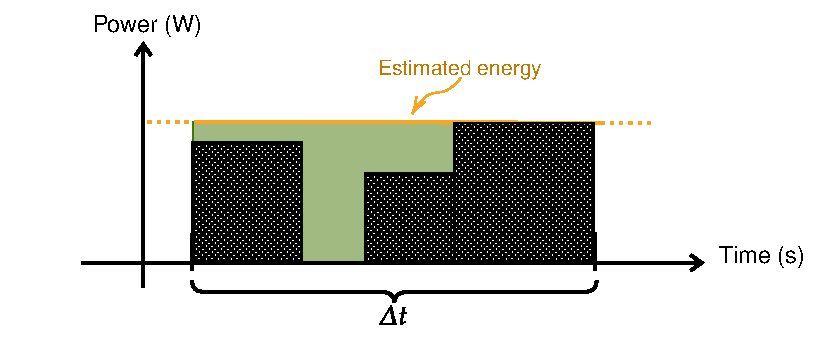
\includegraphics[scale=0.8]{Images/Model/energy_consumption.pdf}
    \caption[Energy consumption comparison between predicted and real.]{Energy consumption comparison between predicted and real. The black boxes are jobs. The green area is the energy predicted, but not used.}
    \label{fig:energy_consumption}
\end{figure}

The renewable production variation comes from the wind and solar variations. 
% This variance comes from the uncertainties presented in Section \ref{sec:weather_uncertainties}. 
These uncertainties can increase or decrease power generation $P_{renew}$. Finally, the scheduler adapts the server configuration to improve the QoS. Since the objective of the scheduling is to maximize the finished jobs, it must modify the offline plan. For example, if a job is running on a server, but the IT offline plan indicates putting this server to sleep, it would kill the job. So, ODM can change this decision, using more energy now and maintaining the job running. Another case is considering the speed given to the job. Letting a job in a server with a slower P-state can increase the execution time ($Ex_j$), violating Constraint \ref{equ:walltime} and killing the job. A way to reduce this possibility is by using Equation \ref{equ:avoid_walltime}. This equation verifies the minimum speed to complete the remaining job's flops. 

\begin{equation}
    (Wall_j - Ex_j) \times D_{s,d} \times F_{s,d} \ge Dfl'_j - Gfl_j
    \label{equ:avoid_walltime}
\end{equation}

Since ODM does not know the job's flops exactly, it can estimate using the walltime. Equation \ref{equ:estimated_job_size} shows a way for estimating $Dfl'_j$, similar to \cite{takizawa2020effect}. $F'_{s}$ is a fixed speed applied to the job. $\epsilon_{u}$ is a user error because the user can overestimate the execution time. We do not consider the walltime underestimation, because this always leads to killing the job (respecting Equation \ref{equ:walltime}). \citeauthor{takizawa2020effect} calculate $\epsilon_{u}$ for each user, using previous users' requests. Even if Equation \ref{equ:avoid_walltime} does not exactly use the real size, it is a good way to balance the states of a job.

\begin{equation}
    \label{equ:estimated_job_size}
    Dfl'_j = wall_j \times F'_{s} \times \epsilon_{u}
\end{equation}

The batteries smooth these variations, providing the power needed in case of underproduction or absorbing the generation excess. At the end of time step $t$, the $SoC(t)$ can be different from the prediction. Therefore, ODM recalculates all future $SoC$ using Equations \ref{equ:battery_energy} and \ref{equ:battery_state_of_charge}. With the $SoC(T)$ updated, Equation \ref{equ:delta_energy} can estimate how far the SoC at the end of the time window will be from the target. This equation gives a value of energy (in kWh). A positive $\Delta E_{bat}$ means that the battery will have more energy than predicted, allowing the scheduler to use this excess to run more jobs or speed up the servers. On the other hand, a negative $\Delta E_{bat}$ means that the battery will have less energy than predicted. In this case, ODM must reduce future usage to approximate $SoC(T)$ to $SoC_{target}$.

\begin{equation}
    \label{equ:delta_energy}
    \Delta E_{bat} = \frac{SoC(T) - SoC_{target}}{100}\times C_{bat}
\end{equation}

Then, ODM calculates how much energy it can compensate, using Equation \ref{equ:energy_battery}. This equation considers the loss in the process of charge/discharge. 

\begin{equation}
    \label{equ:energy_battery}
    E_{comp} = \begin{cases}
        \frac{\Delta E_{bat}}{\eta_{ch}} & \Delta E_{bat} > 0 \\
        \frac{\Delta E_{bat}}{\eta_{dch}} & \Delta E_{bat} < 0 \\
    \end{cases}
\end{equation}

Finally, ODM must modify futures $P_{dch}$ and $P_{ch}$ to use $E_{comp}$. We focus on battery modifications since it is faster to make online decisions on it. Hydrogen is not too reactive. We proposed some ways to deal with it in the following chapters. Since ODM modifies $P_{dch}$ and $P_{ch}$, $P_{prod}$ will also change (see Equation \ref{equ:model_energy}). So, ODM must adapt the IT plan (servers' states $D_{s,d}$) to meet the new $P_{prod}$. The algorithm to modify $D_{s,d}$ on-the-fly is also presented in the following chapters. This modification must respect the Constraint \ref{equ:ITDM_energy_less_envelope}. We name the process of adapting the power plan power/energy compensation or migration. The compensations/migration can be:

\begin{itemize}
    \item Positive: In this case $\Delta E_{bat} > 0$. So, we can increase the battery power usage now or in the future.
    \item Negative: In this case $\Delta E_{bat} < 0$. So, we should reduce the battery power usage now or in the future.
\end{itemize}

Figure \ref{fig:model_compensation} illustrates the positive and negative compensations. Both compensations first observe a variation in battery usage (green box). In positive compensation, it verifies a lower usage in step 1. This reduction makes $\Delta E_{bat} > 0$, so we can increase the battery usage in the future (yellow box in step 4). The negative compensation is the opposite, where we observe a higher usage in step 1 (making $\Delta E_{bat} < 0$), demanding a lower usage in the future. As mentioned before, this variance in battery usage comes from scheduling modifications, server idleness, and renewable production fluctuations.

\begin{figure}[!htb]
    \centering
    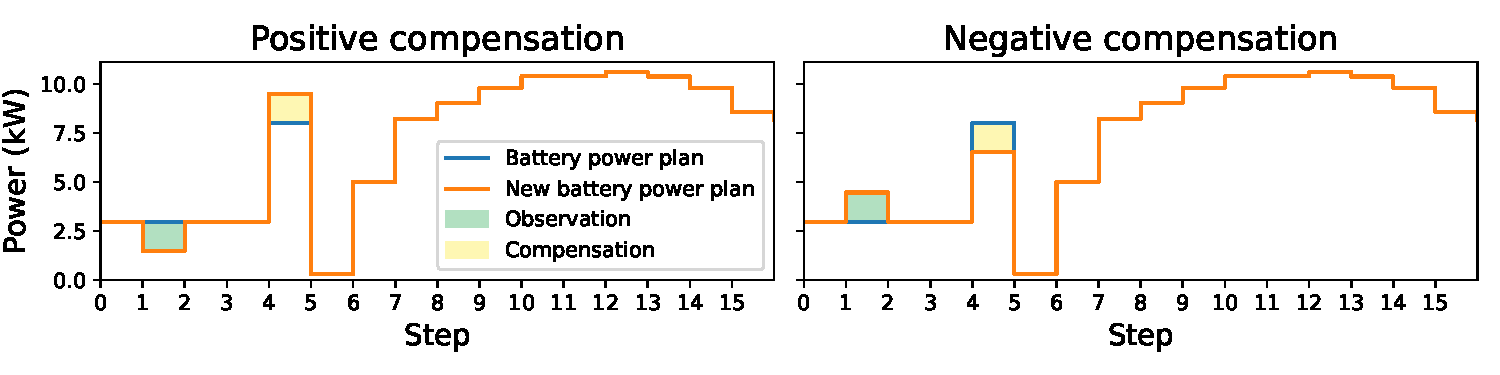
\includegraphics[scale=0.58]{Images/Model/compensation.pdf}
    \caption[Positive and negative compensations]{Positive and negative compensations. We observe a variation in step 1 and compensate it in step 4, according to the compensation type (positive or negative).}
    \label{fig:model_compensation}
\end{figure}

\section{Data}
After describing the models, we describe the data used to simulate our environment. Our simulators expect three data: workload, weather, and platform. We explain the source of each one in the following sections. 

\subsection{Workload Trace}
\label{sec:workload_trace}

Workload trace is a log of job submissions in a resource (servers) provider. Some trace examples are Microsoft Azure \cite{cortez2017resource}, Google \cite{reiss2011google}, and Alibaba \cite{wang2022characterizing}. Regarding batch, \citeauthor{feitelson2014experience} proposed the SWF format, which allows the data center providers to distribute logs to the research community \cite{feitelson2014experience}. In SWF, each line is a job with the fields separated by whitespace. Each line contains the following fields \cite{feitelson2014experience}:
\begin{itemize}
    \item \textit{Job Number}: The job ID starting with 1;
    \item \textit{Submit Time}: The submission time. The first job has 0 as submit time, and the following jobs use the first job as reference (in seconds);
    \item \textit{Wait Time}: How long the job waited in the queue (in seconds);
    \item \textit{Run Time}: The execution time in the data center (in seconds);
    \item \textit{Number of Allocated Processors}: The number of processors allocated to the job (integer);
    \item \textit{Average CPU Time Used}: The time that the job used the CPU. It is the average from all processors (integer);
    \item \textit{Used Memory}: The used memory, also average from all processors (kilobytes);
    \item \textit{Requested Number of Processors}: The number of processors requested by the user (integer);
    \item \textit{Requested Time}: This is the walltime (seconds);
    \item \textit{Requested Memory}: Requested memory per processor  (kilobytes);
    \item \textit{Status}: 1 if the job was completed, 0 if it failed, and 5 if canceled;
    \item \textit{User ID}: The user ID. Can be used to identify different jobs from the same user (integer);
    \item \textit{Group ID}: A group ID (some systems control the group and not the user ID) (integer);
    \item \textit{Executable (Application) Number}: Can link different jobs from the same application (integer);
    \item \textit{Queue Number}: Indicates in which queue the job was allocated (integer);
    \item \textit{Partition Number}: Indicates in which partition the job was allocated. For example, it is possible to use partition numbers to identify which machine in a cluster was used (integer);
    \item \textit{Preceding Job Number}: Indicates the number of a previous job in the workload, such that the current job can only start after the termination of this preceding job (integer);
    \item \textit{Think Time from Preceding Job}: The time between this job and the Preceding Job (seconds);
\end{itemize}

It is not mandatory to insert all information in a SWF file. Currently, Parallel Workloads Archive\footnote{https://www.cs.huji.ac.il/labs/parallel/workload/index.html} has 40 traces in SWF format. We chose the MetaCentrum2 workload trace from the Czech National Grid Organization \cite{klusavcek2015real}. MetaCentrum is a grid with resources in several cities in the Czech Republic. They have 19 clusters with 495 nodes and 8412 cores in total. Nodes are individual machines or servers within a cluster. Each node can have its own set of resources such as CPU, memory, storage, and network connectivity. A core refers to a processing unit within a CPU (Central Processing Unit). Modern CPUs often have multiple cores, allowing them to perform multiple tasks simultaneously. The trace has 5,731,100 jobs from January 2013 to April 2015. Metacentrum does not provide the \textit{Average CPU Time Used}, \textit{Used memory}, \textit{Status}, \textit{Group ID}, \textit{Executable (Application) Number}, \textit{Preceding Job Number}, and \textit{Think Time from Preceding Job} fields. It has different queues according to the job type. The Partition number indicates which cluster executed the job. We do not have more information about the servers, just the number of nodes, cores, and memory.

Figure \ref{fig:metacentrum} illustrates the inter-arrival and execution time distribution for MetaCentrum2. Inter-arrival is the time between job submissions, and execution time is the real runtime. Applying the Kolmogorov-Smirnov test to these data, we observed that both follow a log-normal distribution with p-value = 0.2174 for inter-arrival and p-value = 0.1802 for execution time (excluding 0.003838705\% of jobs as outliers). In the Kolmogorov-Smirnov test, if the p-value is smaller than the chosen significance level (we chose a confidence level of 95\%, so smaller than 0.05), it indicates that there is strong evidence to suggest that the data doesn't follow the specified distribution (both values are higher than the significance level).

\begin{figure}[!htb]
    \centering
    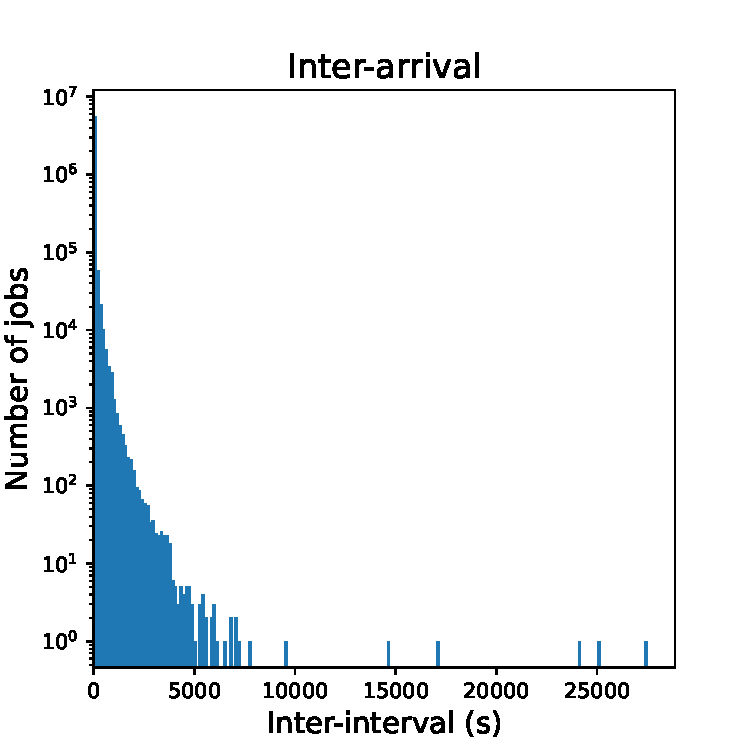
\includegraphics[scale=0.55]{Images/Model/interarrival.pdf}
    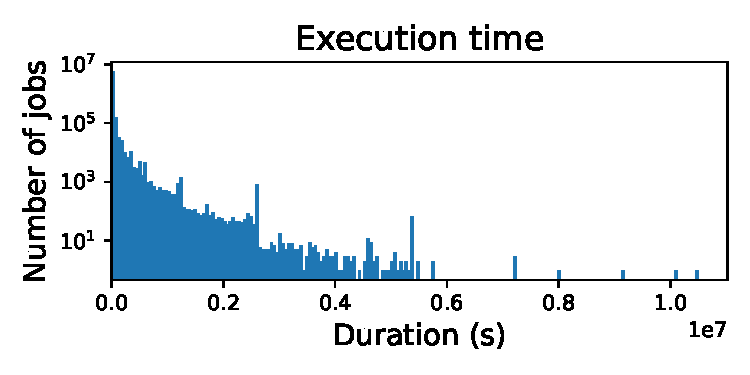
\includegraphics[scale=0.55]{Images/Model/execution_time.pdf}
    \caption{Inter arrival and execution time distribution for MetaCentrum2 workload trace.}
    \label{fig:metacentrum}
\end{figure}

Another aspect of the MetaCentrum2 workload is the \textit{Requested Time} field. This field could be considered as walltime. Nevertheless, MetaCentrum2 defines this field according to the job queue. Consequently, it does not come from the user. We recalculate the walltime using the proposition from \citeauthor{takizawa2020effect} \cite{takizawa2020effect}. Thus, we equally divided the jobs into five groups. Each group estimates the walltime as follows:

\begin{enumerate}
    \item walltime = real execution time $\times$ 5
    \item walltime = real execution time $\times$ 3.333333333
    \item walltime = real execution time $\times$ 2
    \item walltime = real execution time $\times$ 1.428571429
    \item walltime = real execution time $\times$ 1.111111111
\end{enumerate}

This uncertainty complicates the scheduling decisions but it is more realistic. We created two scripts for translating the SWF format to the simulator chosen (see Section \ref{sec:BATSIM}) and Datazero2 Middleware formats. We simulated several possibilities of workload, and each chapter will describe the selection process.

\subsection{Weather Trace}
\label{sec:weather_trace}

Regarding weather, we are interested in the traces of solar irradiance and wind speed, which allow us to estimate power generation using Equations \ref{equ:panel_solar_with_temperature} and \ref{equ:wind_turbines}. NASA's Modern-Era Retrospective Analysis for Research and Applications (MERRA) provides a dataset of solar irradiance and wind speed from any place in the world \cite{rienecker2011merra}. Regarding wind speed, we get the data directly from the MERRA site\footnote{https://power.larc.nasa.gov/data-access-viewer/}. Renewable Ninja\footnote{https://www.renewables.ninja/} is a tool that transforms the weather from MERRA to electricity production \cite{pfenninger2016long, staffell2016using}. Renewable Ninja uses some solar panel models to estimate power generation. We use Renewable Ninja to obtain ground-level solar irradiance because the authors consider cloud cover and aerosols' impact on the irradiance. We chose Toulouse, France as the reference point, getting the data from 2020. After exporting the data, we also translate the output CSV to the simulator chosen (see Section \ref{sec:BATSIM}) and Datazero2 Middleware formats. We took different days from 2020 for our simulations. The following chapters will present the selection process.

\subsection{Platform Configuration}
\label{sec:platform_configuration}

Finally, the last data is the hardware specification. This configuration simulates the real behavior of the different components of a data center, such as servers, storage, network, etc. In this thesis, we focused on the server specification. For simulating a DVFS-enabled server, the following information is necessary:
\begin{itemize}
    \item Sleeping power: Power used to maintain a server sleeping;
    \item Time for on\(\rightarrow\)off transition: Time to turn off a server;
    \item Power for on\(\rightarrow\)off transition: Power to turn off a server;
    \item Time for off\(\rightarrow\)on transition: Time to turn on a server;
    \item Power for off\(\rightarrow\)on transition: Power to turn on a server;
    \item Power idle: Power used when the server is idle;
    \item DVFS states: A list of states containing:
    \begin{itemize}
        \item Power: The power used in the state with all processors busy;
        \item Speed: The speed in the state.
    \end{itemize}
\end{itemize}

We chose to model a data center using the specification from GRID5000 servers. \citeauthor{dacosta:hal-03453537v1} performed experiments in GRID5000 to obtain the data for the DVFS states \cite{dacosta:hal-03453537v1, dacostakeynote}. Some other authors also simulated GRID5000 machines, giving information about their simulation \cite{rais2018quantifying, caux2018optimization, caux2019phase, villebonnet2016energy}. We consolidate these works to create a platform for both the simulator chosen (see Section \ref{sec:BATSIM}) and Datazero2 Middleware. Table \ref{tab:gros} exemplifies the consolidated data for GRID5000's Gros server used in the experiments.

% \begin{table}[!htb]
% \centering
% \caption{Gros definition. The power is for all server's processors busy. The values are from Grid5000's Gros server.}
% \label{tab:gros}
% \begin{tabular}{ll|l}
%     \hline
%     \multicolumn{2}{l|}{Parameter} & Value \\ \hline\hline
%     \multicolumn{2}{l|}{Sleeping power} & 4.5 W \\
%     \multicolumn{2}{l|}{Time on-\textgreater{}off} & 6 s \\
%     \multicolumn{2}{l|}{Power on-\textgreater{}off} & 76.5 W \\
%     \multicolumn{2}{l|}{Time off-\textgreater{}on} & 164 s \\
%     \multicolumn{2}{l|}{Power off-\textgreater{}on} & 110.52 W \\
%     \multicolumn{2}{l|}{Power idle} & 62 W \\ \hline
%     \multicolumn{3}{l}{DVFS states}  \\ \hline 
%     \multicolumn{1}{l|}{State} & Power (W) & Speed per core (Gflops) \\ \hline\hline
%     \multicolumn{1}{l|}{0} & 143.45 & 35.2 \\
%     \multicolumn{1}{l|}{1} & 123.57 & 33.59 \\
%     \multicolumn{1}{l|}{2} & 122.34 & 31.98 \\
%     \multicolumn{1}{l|}{3} & 121.68 & 30.36 \\
%     \multicolumn{1}{l|}{4} & 118.49 & 28.79 \\
%     \multicolumn{1}{l|}{5} & 115.8 & 27.14 \\
%     \multicolumn{1}{l|}{6} & 114.58 & 25.57 \\
%     \multicolumn{1}{l|}{7} & 110.89 & 23.85 \\
%     \multicolumn{1}{l|}{8} & 108.06 & 22.38 \\
%     \multicolumn{1}{l|}{9} & 106.81 & 20.78 \\
%     \multicolumn{1}{l|}{10} & 104.13 & 19.18 \\
%     \multicolumn{1}{l|}{11} & 102.83 & 17.59 \\
%     \multicolumn{1}{l|}{12} & 100.78 & 15.99 \\ \hline
% \end{tabular}
% \end{table}

\begin{table}[!htb]
    \caption[Gros definition]{Gros definition. The power is for all server's processors busy. The values are from Grid5000's Gros server.}
    \label{tab:gros}
    \begin{minipage}{.45\linewidth}
      \centering
      \begin{tabular}{l|l}
        \hline
        Parameter & Value \\ \hline\hline
        Sleeping power & 4.5 W \\
        Time on$\rightarrow$off & 6 s \\
        Power on$\rightarrow$off & 76.5 W \\
        Time off$\rightarrow$on & 164 s \\
        Power off$\rightarrow$on & 110.52 W \\
        Power idle & 62 W \\ \hline
    \end{tabular}
    \end{minipage}%
    \begin{minipage}{.55\linewidth}
      \centering
      \begin{tabular}{l|l|l}
        \hline
        State & Power (W) & Speed per core (Gflops) \\ \hline\hline
        0 & 143.45 & 35.2 \\
        1 & 123.57 & 33.59 \\
        2 & 122.34 & 31.98 \\
        3 & 121.68 & 30.36 \\
        4 & 118.49 & 28.79 \\
        5 & 115.8 & 27.14 \\
        6 & 114.58 & 25.57 \\
        7 & 110.89 & 23.85 \\
        8 & 108.06 & 22.38 \\
        9 & 106.81 & 20.78 \\
        10 & 104.13 & 19.18 \\
        11 & 102.83 & 17.59 \\
        12 & 100.78 & 15.99 \\ \hline
    \end{tabular}
    \end{minipage} 
\end{table}

\section{Simulation}
\label{sec:simulation}

After describing the source of data, we detail our simulation environment. We explain two simulators and the work done to adapt our data for these simulators. We define the different metrics used to evaluate the algorithms in the following chapters.

\subsection{Batsim Simulator}
\label{sec:BATSIM}

Batsim is an infrastructure simulator that enables the study of resource management policies \cite{batsim_jsspp16}. This simulator is based on the well-known Simgrid \cite{casanova2001Simgrid}. The Batsim protocol helps to develop scheduling and resource management algorithms without Simgrid knowledge. The protocol works via a socket and includes the following events:
\begin{itemize}
    \item Bidirectional (Batsim$\rightarrow$Scheduler and Scheduler$\rightarrow$Batsim):
    \begin{itemize}
        \item \textit{QUERY}: It has two queries. First, in the \textit{consumed\_energy} query, the scheduler asks Batsim about the total consumed energy (from time 0 to now). On the other hand, in the \textit{estimate\_waiting\_time}, Batsim demands the scheduler what would be the waiting time of a potential job;
        \item \textit{ANSWER}: The \textit{QUERY} answer;
        \item \textit{NOTIFY}: This event allows a peer to notify something to its counterpart. This message can be a specific message from an external event.
    \end{itemize}
    \item Batsim$\rightarrow$Scheduler:
    \begin{itemize}
        \item \textit{JOB\_SUBMITTED}: A new job was submitted;
        \item \textit{JOB\_COMPLETED}: The job has completed its execution;
        \item \textit{JOB\_KILLED}: The job was killed;
        \item \textit{RESOURCE\_STATE\_CHANGED}: The state of a resource (server) changed;
    \end{itemize}
    \item Scheduler$\rightarrow$Batsim:
    \begin{itemize}
        \item \textit{EXECUTE\_JOB}: Execute the job in the servers;
        \item \textit{KILL\_JOB}: Kill the running job;
        \item \textit{SET\_RESOURCE\_STATE}: Set the state of a resource (server);
    \end{itemize}
\end{itemize}

These are some messages of the protocol (the entire protocol is in Batsim documentation\footnote{https://batsim.readthedocs.io/en/latest/protocol.html}). The messages \textit{QUERY} and \textit{ANSWER} enable the scheduler to receive IT energy consumption. The scheduler uses the \textit{JOB\_SUBMITTED}, \textit{JOB\_COMPLETED}, \textit{JOB\_KILLED}, \textit{EXECUTE\_JOB}, and \textit{KILL\_JOB} messages to control the jobs. Finally, the \textit{SET\_RESOURCE\_STATE} and \textit{RESOURCE\_STATE\_CHANGED} allow server configuration. However, Batsim does not provide the electrical management of renewable sources and energy storage. Considering renewable sources, the main objective is receiving power production. Therefore, we applied Equations \ref{equ:wind_turbines} and \ref{equ:panel_solar_with_temperature} on the data from Section \ref{sec:weather_trace}, resulting in a time series of power production. Then, we create a file with several JSON lines:

\begin{lstlisting}[language=json,firstnumber=1]
    {"type": "user_specific_type", "timestamp": 0, "power_available": 0.0}
    {"type": "user_specific_type", "timestamp": 300, "power_available": 460.4}
    {"type": "user_specific_type", "timestamp": 600, "power_available": 5172.26}
\end{lstlisting}

Batsim reads this file and sends at each "timestamp" a \textit{NOTIFY} message. Then, we parse the JSON in the message, taking the power available. $\Delta t$ defines the interval between messages. The scheduler does not know all the events in this JSON file, receiving them just when the simulation arrives at the "timestamp". Regarding energy storage, we implemented two classes to simulate them. The first class is for the battery and uses Equations \ref{equ:battery_energy} and \ref{equ:battery_state_of_charge} to estimate the state of charge. The second class is for hydrogen and implements Equations \ref{equ:hydrogen_electrolyzer}, \ref{equ:hydrogen_fuel_cell}, and \ref{equ:hydrogen_level}. The energy storage implementation must respect the following constraint:

\begin{equation}
    \label{equ:energy_diff}
    ((P_{renew} + P_{dch} + P_{fc} - P_{ez} - P_{ch}) \times \Delta t \times 1000) - E_{tot} = 0
\end{equation}

Constraint \ref{equ:energy_diff} indicates that the difference between energy production ($(P_{renew} + P_{dch} + P_{fc} - P_{ez} - P_{ch}) \times \Delta t \times 1000$) and the energy expended by the IT ($E_{tot}$) must be equal to zero. $P_{renew}$ comes from the JSON input with no modifications. $E_{tot}$ is calculated using \textit{QUERY} and \textit{ANSWER} messages. Since it returns the total energy expended (from 0 to now), we calculate the difference between two \textit{QUERY} calls. So, the simulator balances $P_{dch}$,  $P_{fc}$, $P_{ez}$, and $P_{ch}$. In the default implementation, the simulator first adapts the battery ($P_{dch}$ and $P_{ch}$), and, just if necessary, it changes the hydrogen ($P_{fc}$ and $P_{ez}$).  However, it depends on the implementation (e.g., if the offline plan indicates something different). This simulation respects the boundaries \ref{equ:discharge_boundary}, \ref{equ:charge_boundary}, \ref{equ:fuelcells_boundary}, and \ref{equ:electrolyzer_boundary}.

Another input for Batsim is the platform file. Batsim uses the Simgrid platform format\footnote{https://simgrid.org/doc/latest/Platform.html}. Using the results from Section \ref{sec:platform_configuration}, we created a script to generate this file with all DVFS states. This script receives the server parameters (e.g., Table \ref{tab:gros}) and the number of nodes from this server. It can create homogeneous and heterogeneous data centers according to the user specification. Finally, the last input for Batsim is the workload file. Batsim simplifies the workload definition of batch jobs. We focused on the Homogeneous Parallel Task kind of application in the experiments. In this application type, we define the amount of floating-point operations (flops) to execute on each machine. Here, we create another script to translate the SWF format (from Section \ref{sec:workload_trace}) to Batsim JSON format. An example of a workload file is:

\begin{lstlisting}[language=json,firstnumber=1]
{
    "jobs": [
        {
            "id": "0",
            "profile": "profile_1",
            "res": 1,
            "subtime": 773,
            "walltime": 9112
        }
    ],
    "profiles": {
        "profile_1": {
            "cpu": 163137000000000,
            "type": "parallel_homogeneous"
        }
    },
}       
\end{lstlisting}

In this example, we have only one job with the id equal to 0. This job is submitted after 773 seconds from the simulation beginning (\textit{"subtime": 773}), with a walltime of 9112 seconds (\textit{"walltime": 9112}), and requests one machine (\textit{"res": 1}). The scheduler only knows these fields. The profile field indicates the number of flops to execute. Therefore, the job must calculate 163137000000000 flops. The real execution time is \textit{cpu} divided by the speed of the server which runs this job. The script estimates the field \textit{cpu} by the execution time in SWF multiplied by a server's average speed. We defined the average speed considering the servers in our data center. We took a median DVFS state's speed, avoiding over/underestimating. This estimation is necessary because SWF does not provide any metric of the real computation. All experiments in this thesis use Batsim as the simulator. In parallel, we implement our algorithms in Datazero2 Middleware.

\subsection{Datazero2 Middleware}

The Datazero2 project proposes a middleware to integrate all components from Figure \ref{fig:model}. This middleware has all electrical and IT components, external event integrations, and decision modules. It works on two coding languages: Python and C++. It depends on different frameworks, such as:
\begin{itemize}
    \item ActiveMQ 5.14.4;
    \item C++:
    \begin{itemize}
        \item Protobuf 3.21.8;
        \item Apache APR 1.7.4;
        \item ActiveMQ C++ library 3.9.5;
        \item Simgrid 3.27;
    \end{itemize}
    \item Python:
    \begin{itemize}
        \item Stomp 8.1
        \item Protobuf 3.20.3
        \item Pandas
        \item Pulp
    \end{itemize}
\end{itemize}

Some modules work in Python, and some in C++. The messages from the modules are exchanged via ActiveMQ, using Protobuf as protocol. Simgrid is used to simulate the IT side. The electrical side is implemented using the same rules presented in this thesis. This middleware is still in development by different actors in the project. During this thesis, we worked on the ODM implementation. The results from the Batsim simulations are being implemented in the middleware. 

However, we helped with all these dependencies management, allowing every project's partner to execute the middleware on their computers. Therefore, we create a docker version of the middleware. We create three containers: ActiveMQ, C++, and Python. The ActiveMQ provides the message BUS for all the modules. C++ implements the Simgrid and some modules (e.g., ODM). Python has the electrical control and other modules (e.g., ITDM and PDM). We create a docker-compose script that installs and compiles everything. We included some advanced parameters for developers for coding inside docker without the need to rebuild everything.

Regarding the middleware's simulation input, some changes were done. The weather data is passed directly to the middleware, which applies the equations to transform weather into power. Even if it uses Simgrid (so, same platform file format), the middleware divides this file into two files: Model and Machines. The Model file defines the DVFS states, including a model id. The Machine file indicates all the servers, linking each one to a model id. This division simplifies the modifications in the model. So, we create a new version of the platform script, allowing choose between Batsim or Datazero2 middleware. Finally, the workload file is not JSON but XML. We also create a new version of our script to migrate from SWF to Datazero2 middleware XML.

\subsection{Metrics}

In this section, we present the metrics used in this thesis. We evaluate four aspects in this thesis: Jobs finished, storage state at the end of the time window, wasted energy, and bounded slowdown. The first objective is to increase the number of finished jobs and reduce the number of killed jobs. It is possible to have a high number of finished jobs and a high number of killed jobs in aggressive scheduling, where the scheduler starts jobs even if it is not possible to finish them. Each job can finish in one of five states: 

\begin{enumerate}
    \item Finished: Jobs that finished their computation before the walltime;
    \item Postponed: Jobs postponed to the next time window;
    \item Reached walltime: The jobs that reached the walltime because they do not finish all the computation due to the servers speed;
    \item Not completely finished: The jobs that were not finished completely because they are still running at the end of the time window;
    \item Killed: The killed jobs.
\end{enumerate} 

Therefore, we present the absolute number of jobs in each state at the end of the simulation. In addition, we introduce this metric considering the size of the job ($Dfl_j \times R_j$). The size of the job shows the impact of the decisions in bigger and small jobs. The second aspect is the algorithms must end the time window with the storage levels as close as possible to the planned. This means the algorithms can not "cheat" by using more storage than planned. As explained before, finishing close to the target levels helps to plan the next time window. We present a metric of the distance from the target. This distance can be positive (save more energy) or negative (use more energy). For battery, we present it as the \% difference of target SoC, and for hydrogen, we present it as the kg difference of target LoH.

The third metric is wasted energy. We consider wasted energy the energy expended not computing finished jobs, englobing, for example, the energy used in killed jobs, turning on/off servers, and letting servers idle. This metric is present as kWh. Finally, the fourth metric is the bounded slowdown. This metric is the same as presented in Equation \ref{equ:slowdown}. The bounded slowdown is a difficult metric to compare in executions without the same number of jobs finished. For example, starting and killing a job in the sequence will result in a very low slowdown. On the other hand, maintaining jobs running will make the jobs in the queue wait for more time, which impacts directly on the slowdown. So, we will analyze this metric with precaution.

\section{Conclusion}
This chapter focused on presenting the model, data, and simulation utilized in the remainder of this thesis. The aim is to provide the basis to understand the following chapters. The model introduces all aspects of offline decisions. This offline module builds a plan for the online module. The online model considers the offline as a guide but improves this plan according to the real events. Moreover, the online model considers job scheduling in the decision process. Then, we describe the work done in the data for the simulations. This work includes workload, weather, and platform information. Finally, we explained simulation tools. We detailed the modifications in Batsim to use renewable energy and energy storage. Moreover, we present the metrics used in this thesis to compare the different approaches.

The next chapter introduces the first heuristic to deal with power compensations, trying to improve QoS. After that, Chapter \ref{cha:learning_power_compensations} proposes a model for learning the best power compensations. Finally, Chapter \ref{cha:heuristic} presents our final heuristic, using predictions to make better decisions.